\chapter{Experimental Details}\label{chap:exp_details}

\section{Substrate Preperation}\label{sec:sample_prep}
Using degenerately doped \ac{SiO2} wafers that are $270\unita{nm}$ thick as pictured in fig.~\ref{fig:plain_wafer} there are several preliminary steps needed prior to device fabrication. For easy indentification of locations on the substrate alignment marks are placed on the wafer using photolithography. There is a main alignment mark pictured in fig.~\ref{fig:main_alignment} (REALLY ONLY WANT TO REF A,B) which allows for quicker indentification during electron beam lithography, for example. The alignment marks are in a grid pattern with the coordinate $\left(0,0\right)$ at the center, stretching to $\left(\pm 6,\pm 6\right)$ in both the right and left directions. In each of these coordinate locations there smaller alignment marks evenly spaced within them as shown in fig.~\ref{fig:main_alignment} (FIGURE OUT HOW TO REF SUBFIGS, HERE WE WANT TO REF (c,d)). Next, \ac{Au} is deposited on the surface of the wafer, a process that will be explained in more detail in sec.~\ref{sec:device_fabrication}.
\begin{figure}[ht]
	\centering
	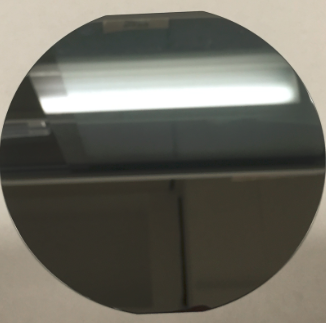
\includegraphics[height=3cm,width=3cm]{figs/experimental/plain_wafer}
	\caption[Plain wafer]{Plain wafer}
	\label{fig:plain_wafer}
\end{figure}
\begin{figure}[ht]
	\centering
	\subfigure[Main alignment mark at 5x magnification]{
		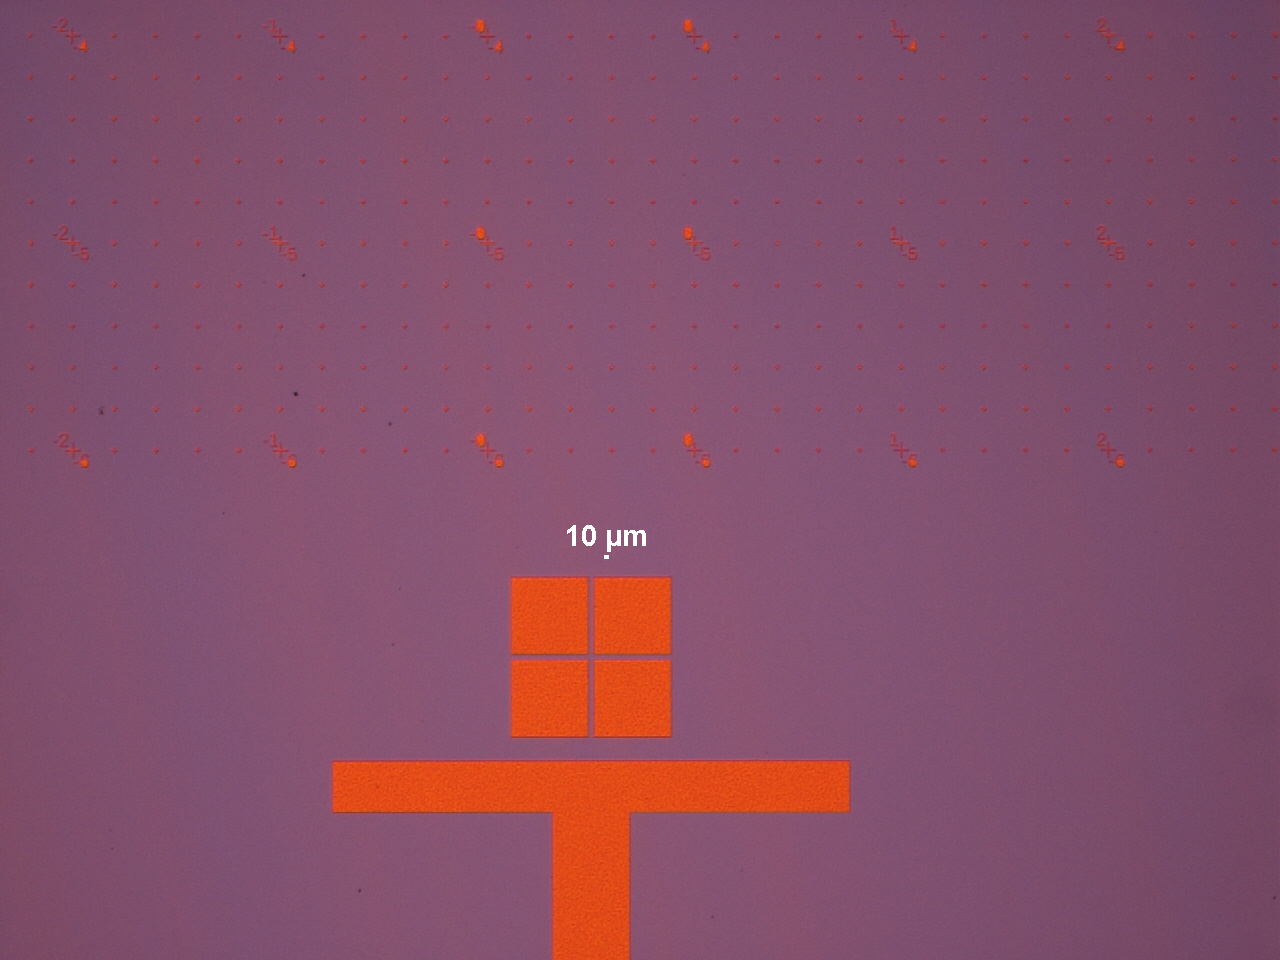
\includegraphics[height=4cm,width=5cm]{figs/experimental/main_alignment_5x}
		\label{fig:main_alignment_5x}
		}
	\quad
	\subfigure[Main alignment mark at 10x magnification]{
		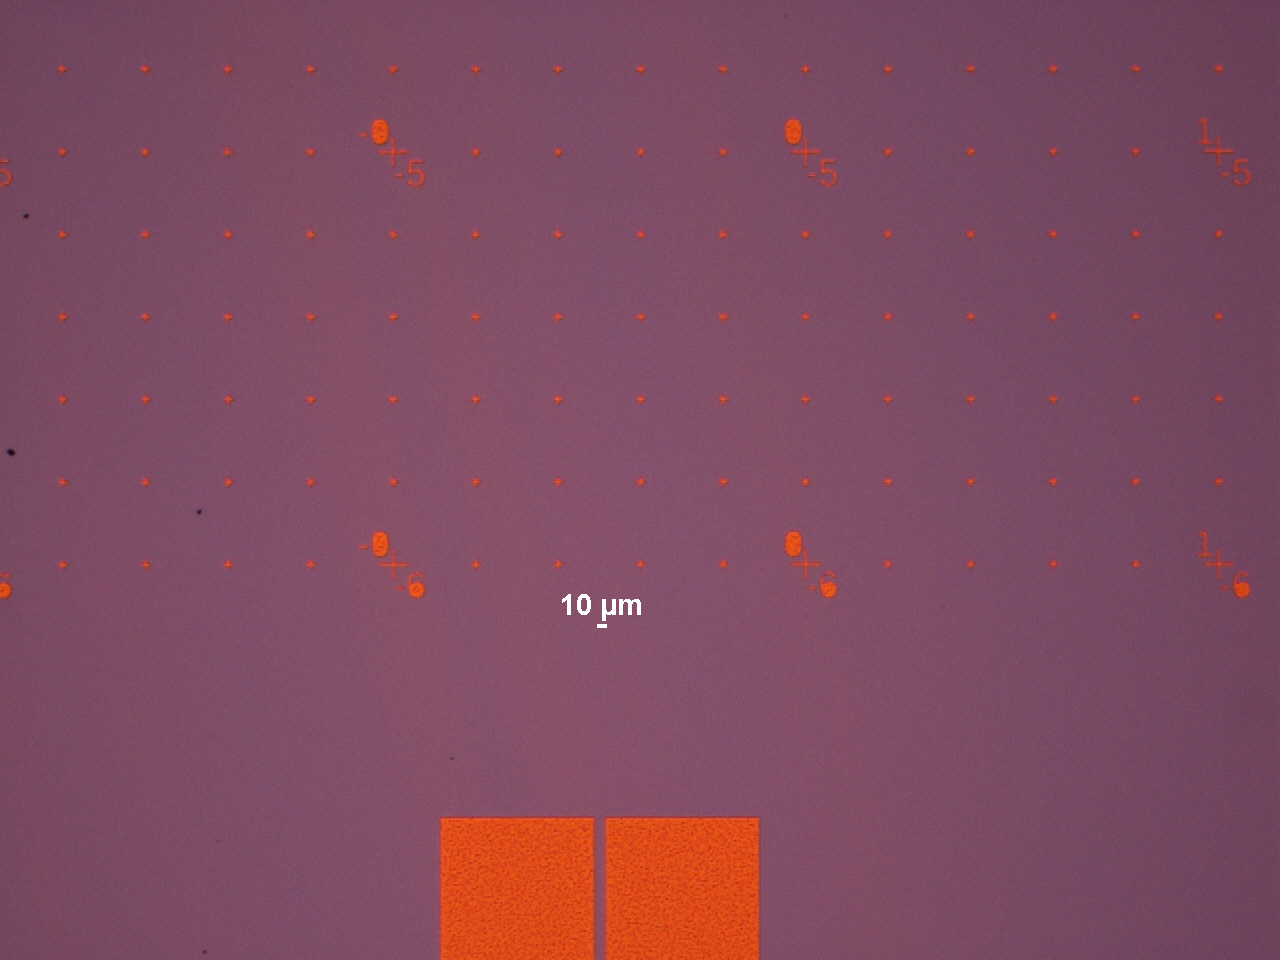
\includegraphics[height=4cm,width=5cm]{figs/experimental/main_alignment_10x}
		\label{fig:main_alignment_10x}
		}

	\subfigure[Coordinate mark $\left(0,-5\right)$ at 50x magnification]{
		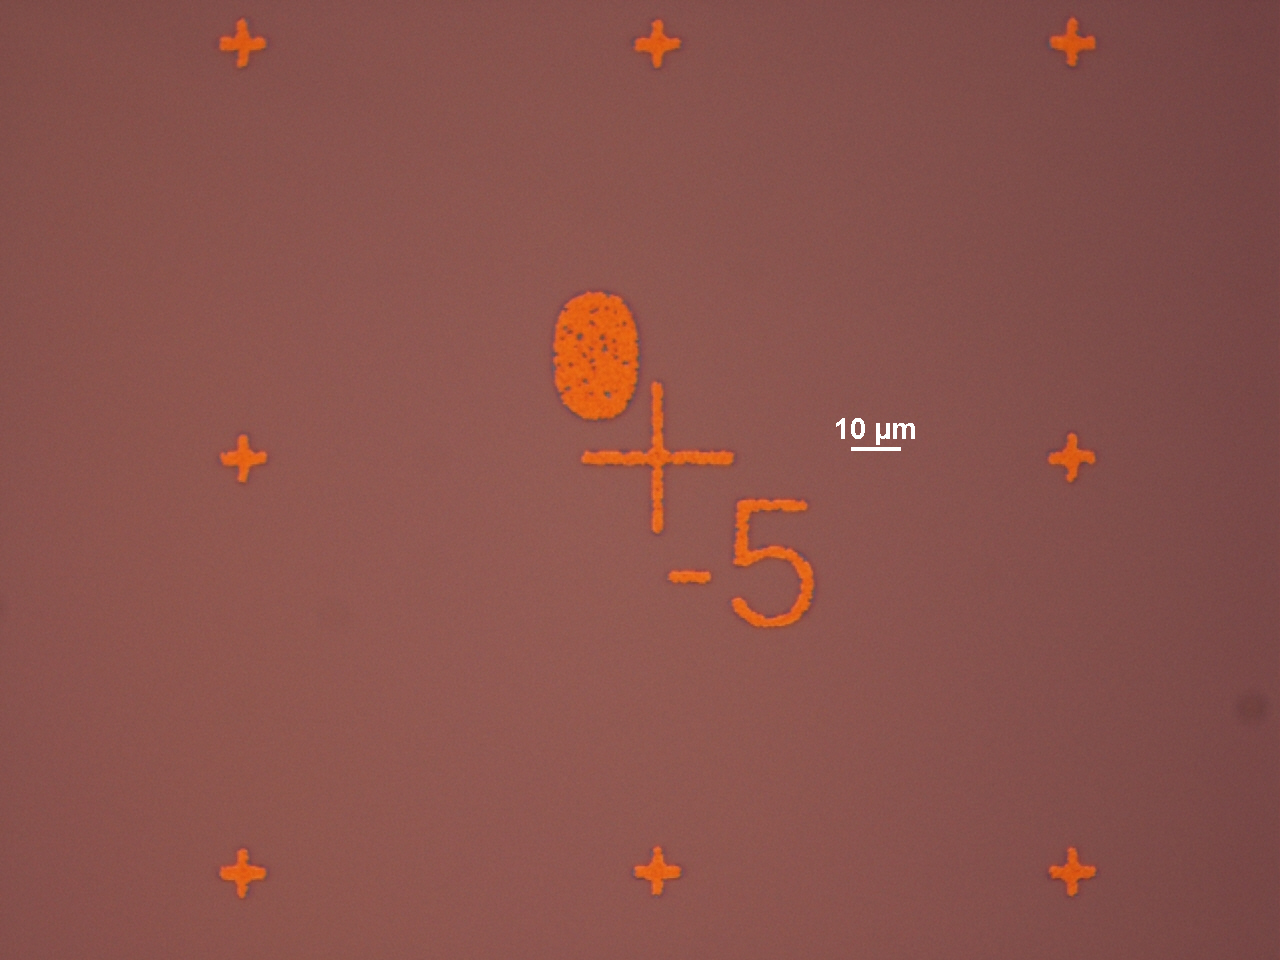
\includegraphics[height=4cm,width=5cm]{figs/experimental/main_alignment_50x}
		\label{fig:main_alignment_50x}
		}
	\subfigure[Coordinate mark $\left(0,-5\right)$ at 100x magnification]{
		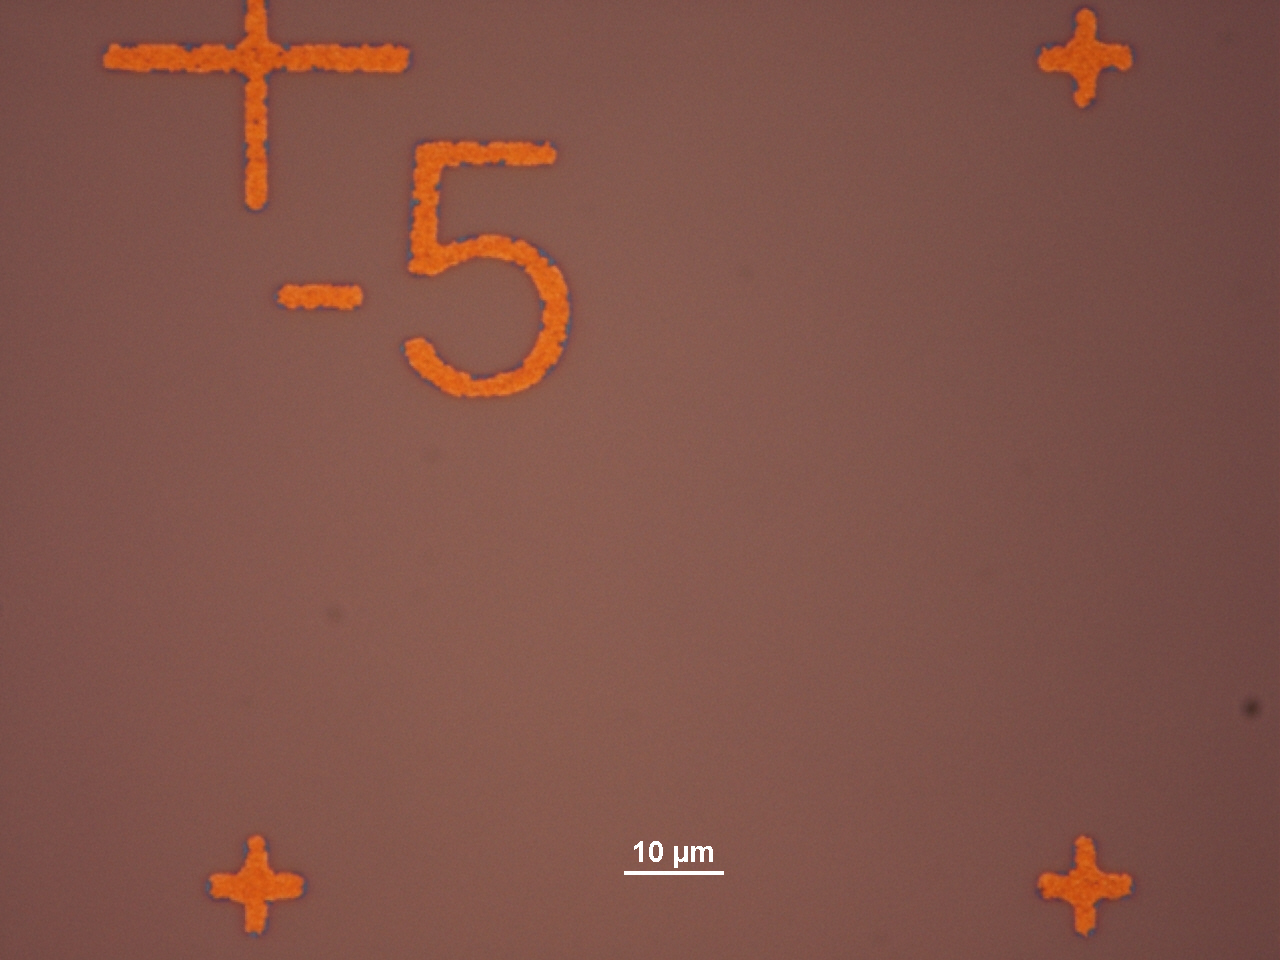
\includegraphics[height=4cm,width=5cm]{figs/experimental/main_alignment_100x}
		\label{fig:main_alignment_100x}
	}
	\caption[Alignment marks at varying magnifications]{Main alignment mark and a coordinate point on a substrate at various magnifications}
	\label{fig:main_alignment}
\end{figure}

\subsection{Substrate Cleaning}\label{subsec:cleaning}
Beginning with a cut \acs{SiO2} substrate with a deposited \acs{Au} layer. To remove the \acs{Au} layer, the substrate is first soaked in acetone for approximately 5-10 minutes then washed using \ac{IPA} and dried with \ac{N2} gas. Next, the substrate in placed in acetone and sonicated for 15 minutes. Then sonicated once more but in \acs{IPA} this time with a repition of washing and drying step using \ac{IPA} and \acs{N2} as described above in between each sonication. In order to remove and remaining organic matter on the surface of the substrate, the substrate is annealed under vacuum at $600^\degree\unita{C}$ for 10 minutes and passing forming gas for 2 of the 10 minutes. Forming gas is a mixture of \ch{H2} and an inert gas, usually \ch{N2} \cite{Choi_AppPhysLett2004}. In addition to annealing the substrate for cleanliness, in certain cases when a higher degree of cleanliness is desired the substrate can be treated with oxygen plasma cleaning. 

\section{Exfoliation}\label{sec:exfoliation}
To synthesize samples the most common and often most effective method used is mechanical exfoliation, a technique made famous by the 2004 Novoselov et al. paper. The process involves using Scotch tape to repeatedly cleave layers of \acs{MoS2} or some other TMD. Starting with a crystal of a particular TMD, placing it on a piece of Scotch tape. Then taking another piece of tape and pressing in on the crystal that is on the first piece of tape, being sure to press hard and firm on the crystal. The tape is then lifted up and this process is repeated until the whole piece of tape is filled with small samples of the TMD. At the end of this process it is expected that there are a wide range of mixture of sample sizes in terms of area and in term of thickness as well, where thicknesses of $<3\unita{nm}$ are not uncommon. To better characterize the samples the optical microscope can be used to do so.
\\ \\
\noindent The main challenge that exists with this method is the ability to synthesize a high yield of monolayer samples. This does not seem to be much of a challenge when it comes to graphene and some other TMDs, but with regard to \acs{MoS2} this is not so simple. Based on recently published literature in an effort to increase the yield of monolayer \acs{MoS2} various methods and techniques were tested and modified accordingly \cite{Huang_et_al_ACSnano2015}. In this modified method an additional step to cleaning the substrate is added in which it undergoes oxygen plasma cleaning for 10 minutes to ensure the cleanliness of the substrate`s surface. To promote more bonding between the substrate and the samples, the substrate is first heated at $300^\degree\unita{C}$ for 10 minutes without any samples on it. During this process the normal cleaving of sample on tape from crystal taking place. Once the substrate is done heating the tape containing sample is immediately placed on the substrate and pressed firmly for several minutes. Then the substrate (with the tape still on it) is placed on a glass slide and is heated at around $85^\degree\unita{C}$ for five minutes. Next, the substrate (with tape) is removed from heat and the tape slowly peeled back from the substrate. The result should be a much higher yield of $<3\unita{nm}$ samples of larger surface area, and several trilayer, bilayer, and a few monolayer samples. (ADD PICTURES OF EACH STEP)
\\ \\
\noindent Most commonly \acs{SiO2} substrates are the main items that are exfoliated onto. However, depending on the material being synthesized, this may not always be the case. In cases where samples of \hbn or in the event that the thickness of the synthesized sample is not of great importance and can to tolerated up to $20-30\unita{nm}$, \ac{PDMS} is exfoliated onto instead of \acs{SiO2} substrates. The resulting samples are of varying thickness, on average around $20\unita{nm}$. Thin samples (usually trilayer and above) can be made using this method of \acs{PDMS}, however, these samples tend to have small surface area and lack uniformity which poses problems as to their usability. As such, this remains an effective method for obtaining samples in which thickness is not the main concern. Once the samples have been optically characterized, the sample(s) on \acs{PDMS} must be transferred to a \acs{SiO2} substrate.

\section{Device Synthesis}\label{sec:synthesis}
\subsection{\acs{PDMS} Transfer}\label{subsec:pdms_transfer}
\begin{figure}[ht]
	\centering
	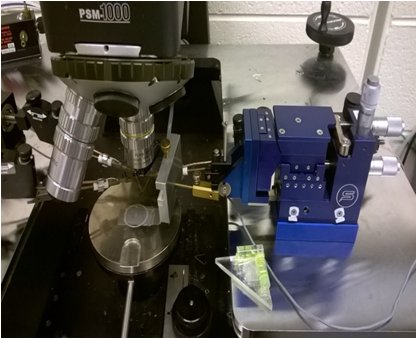
\includegraphics[height=5cm,width=5cm]{figs/experimental/transfer_stage_setup}
	\caption[Transfer stage setup]{Transfer stage setup}
	\label{fig:transfer_stage_setup}
\end{figure}
\subsection{Polycarbonate Pickup Method}\label{subsec:pc_pickup}

\section{Characterization}\label{sec:characterization}
\subsection{Optical Characterization}\label{subsec:characterization_optical}
\begin{figure}[ht]
	\centering
	\begin{minipage}[b]{0.45\linewidth}
		\centering
		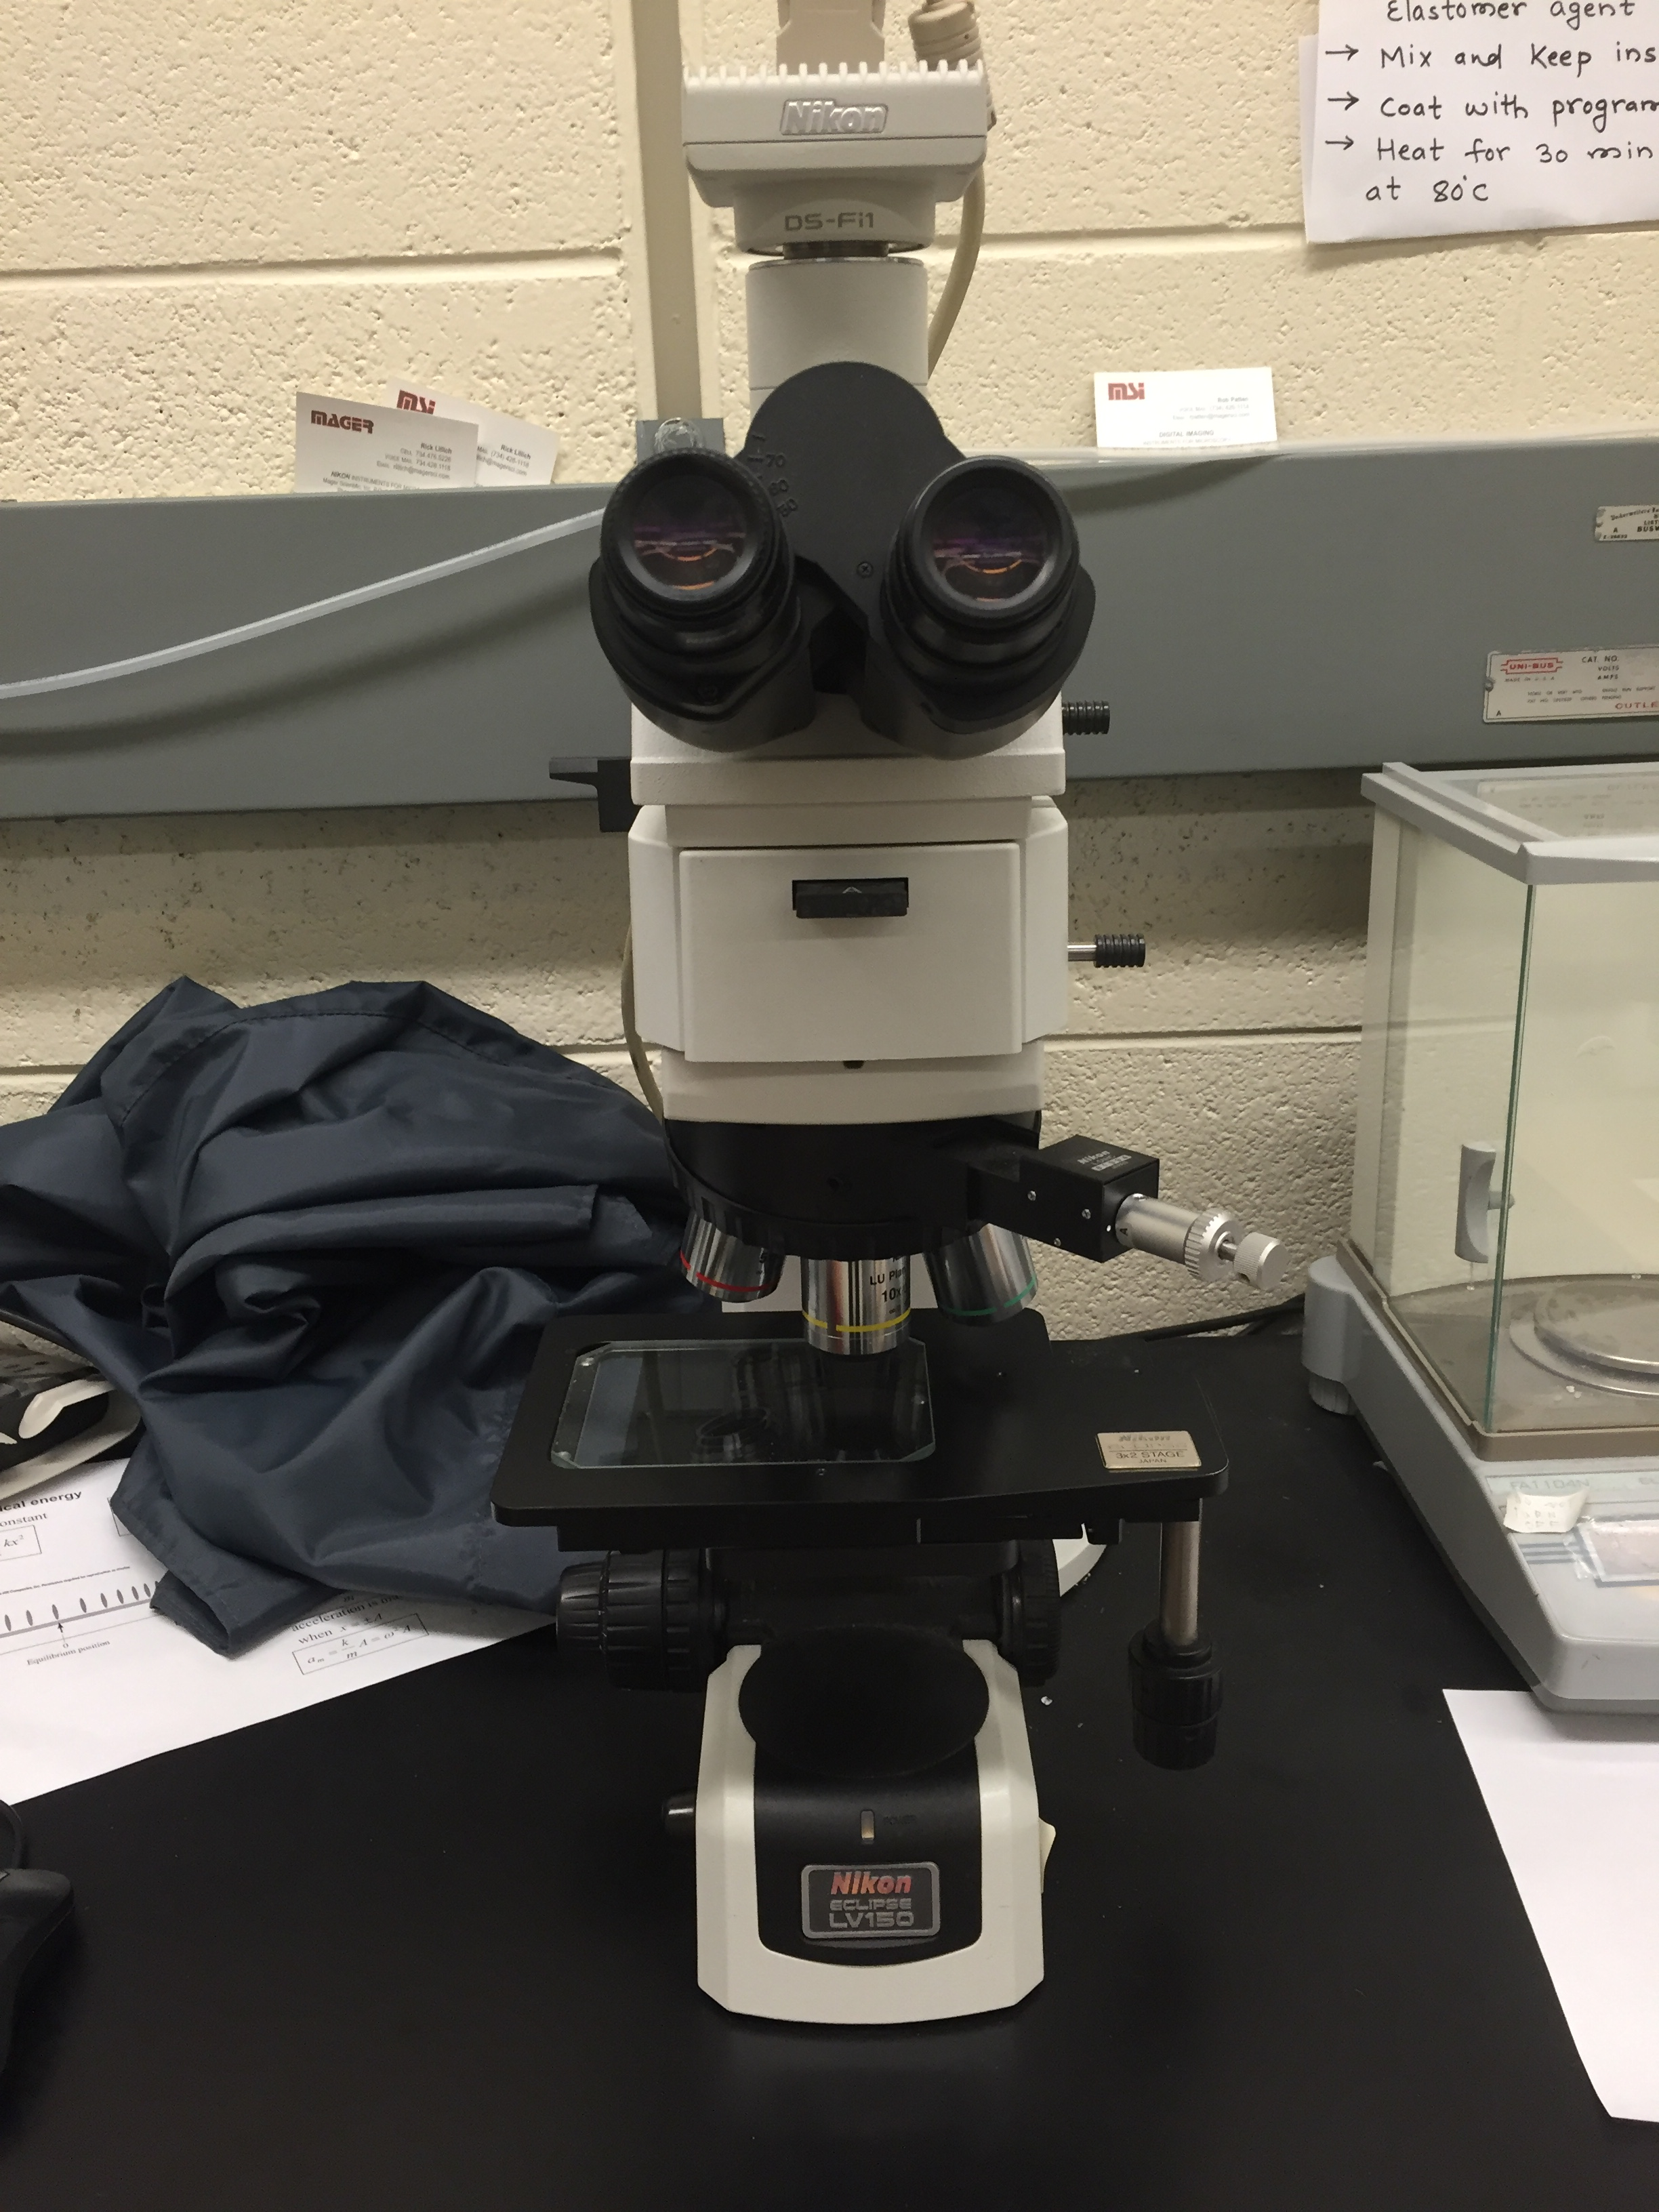
\includegraphics[height=4cm,width=5cm]{figs/experimental/optical_microscope_front_view}
		\caption[Optical microscope front view]{Optical microscope front view}
		\label{fig:optical_microscope_front_view2}
	\end{minipage}
	\qquad
	\begin{minipage}[b]{0.45\linewidth}
		\centering
		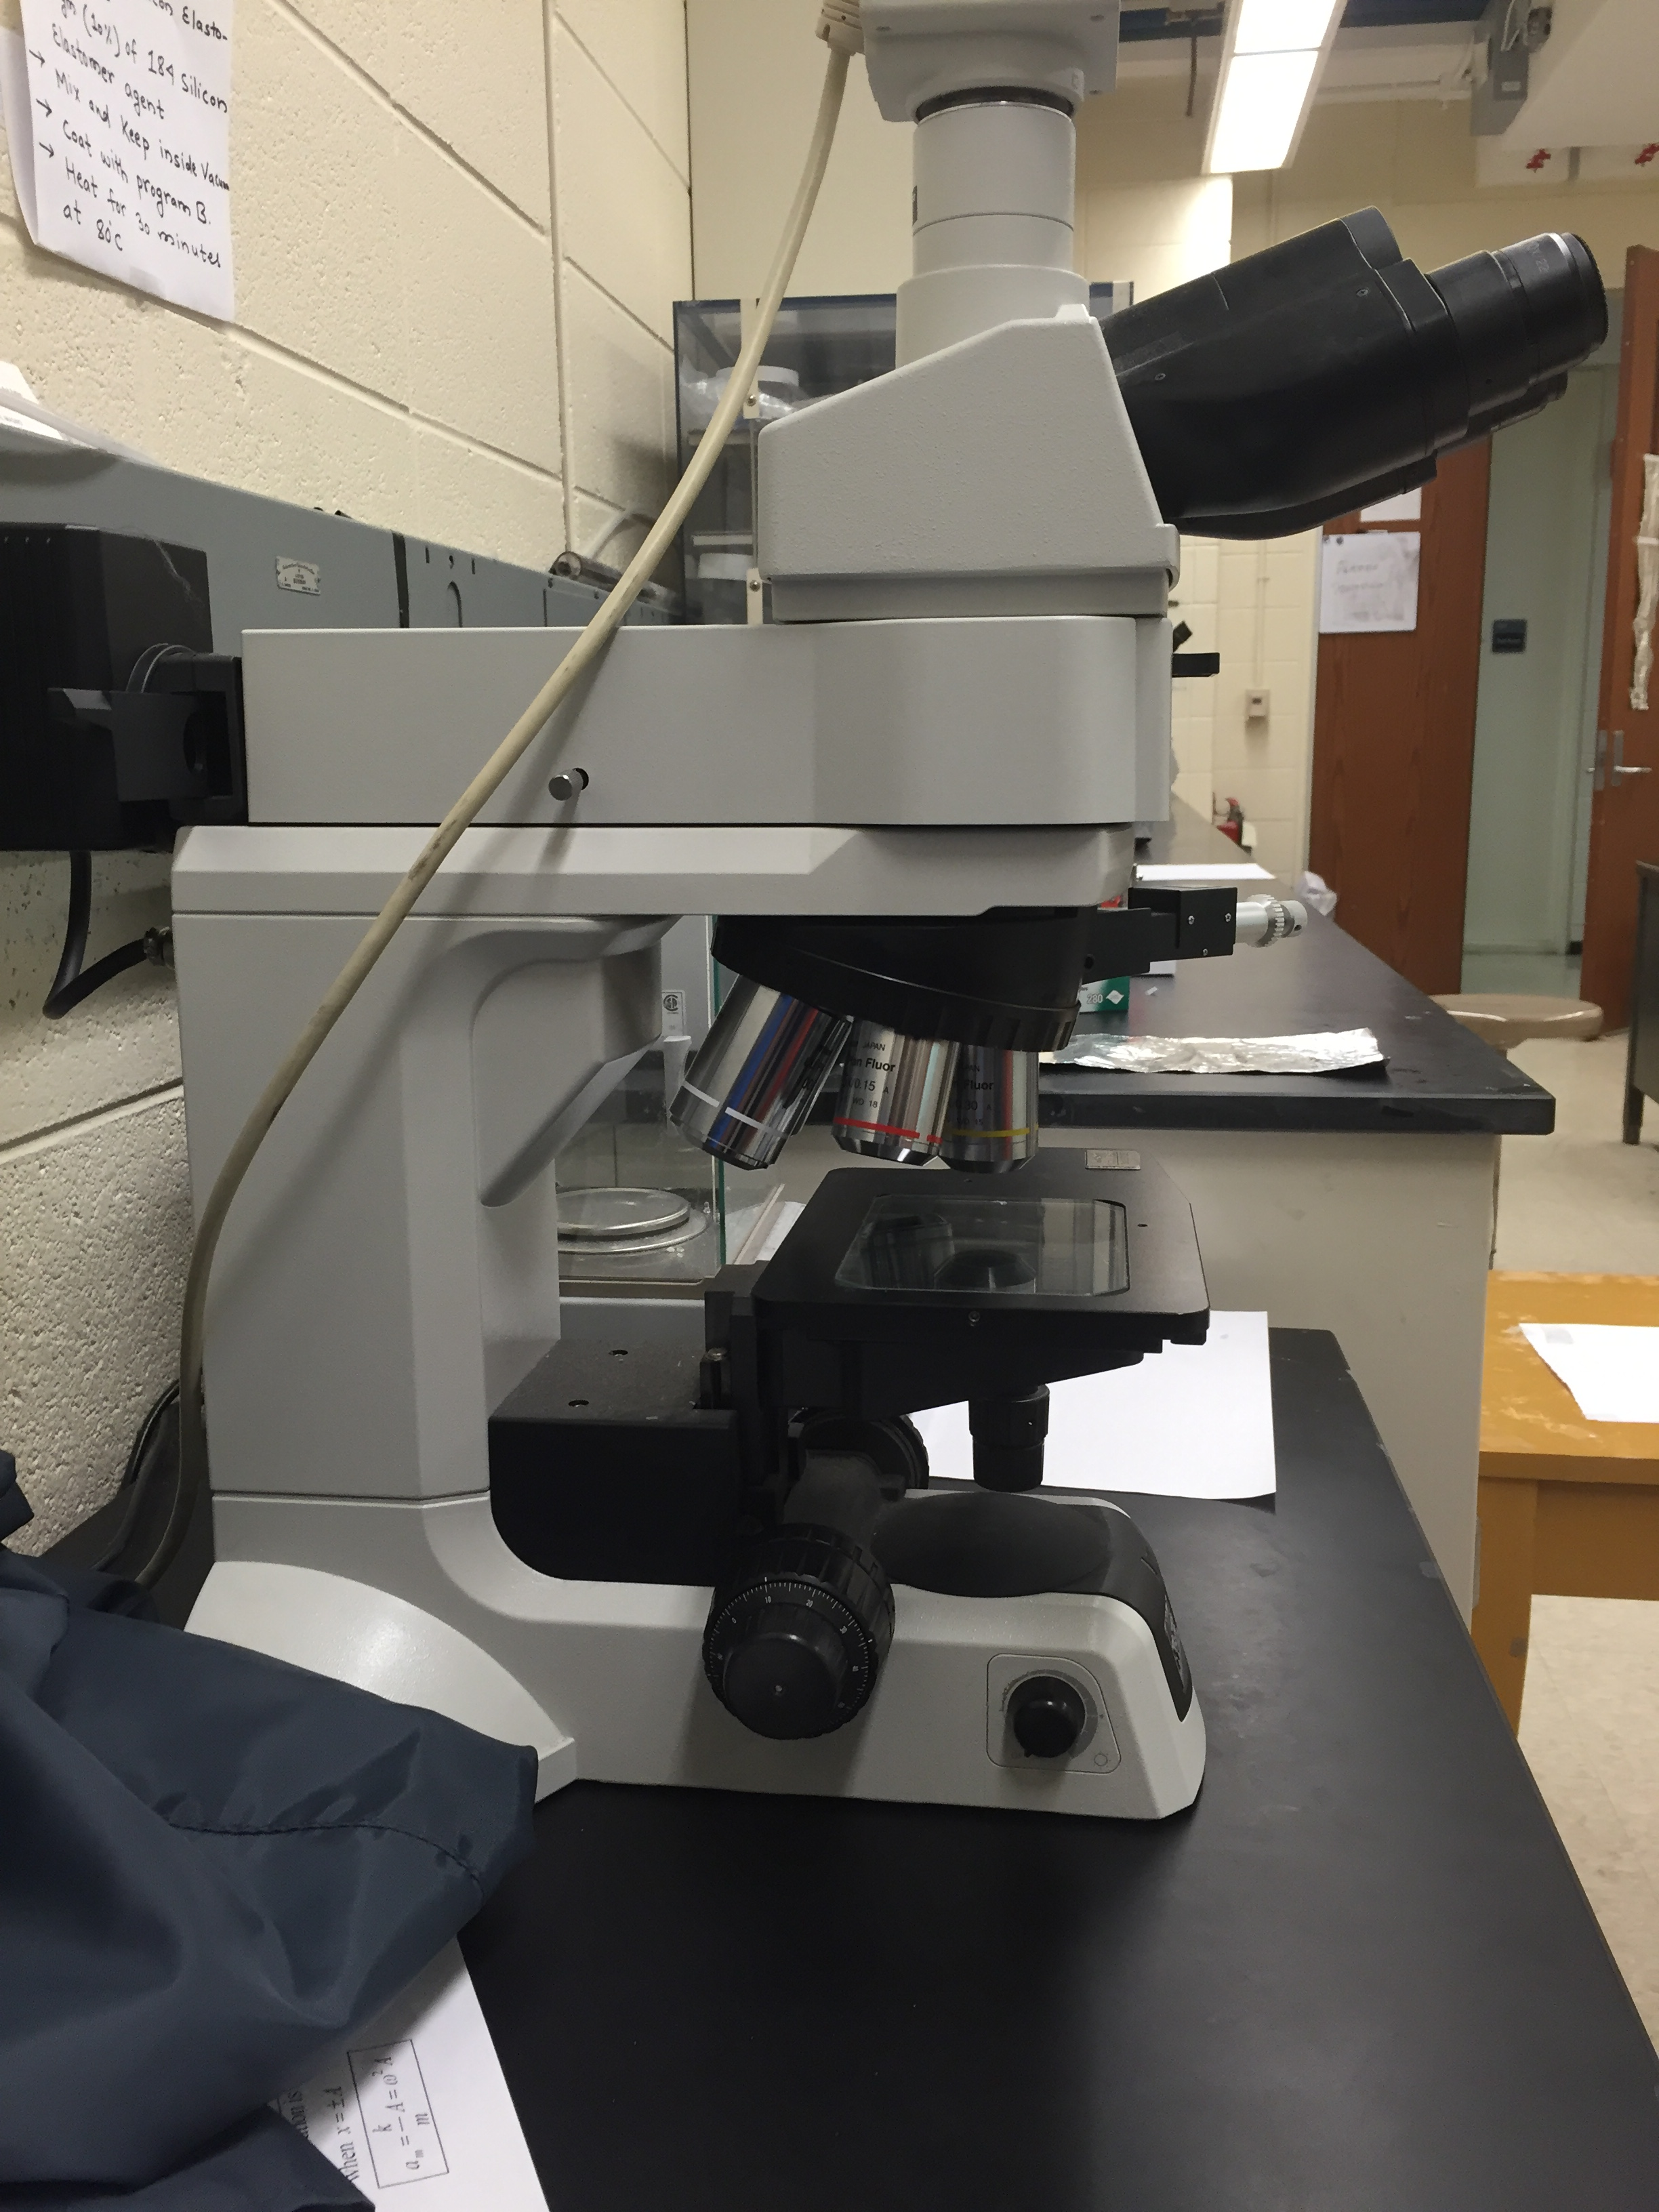
\includegraphics[height=4cm,width=5cm]{figs/experimental/optical_microscope_side_view}
		\caption[Optical microscope side view]{Optical microscope side view}
		\label{fig:optical_microscope_side_view}
	\end{minipage}
\end{figure}

\subsection{AFM Characterization}\label{subsec:characterization_afm}
\begin{figure}[ht]
	\centering
	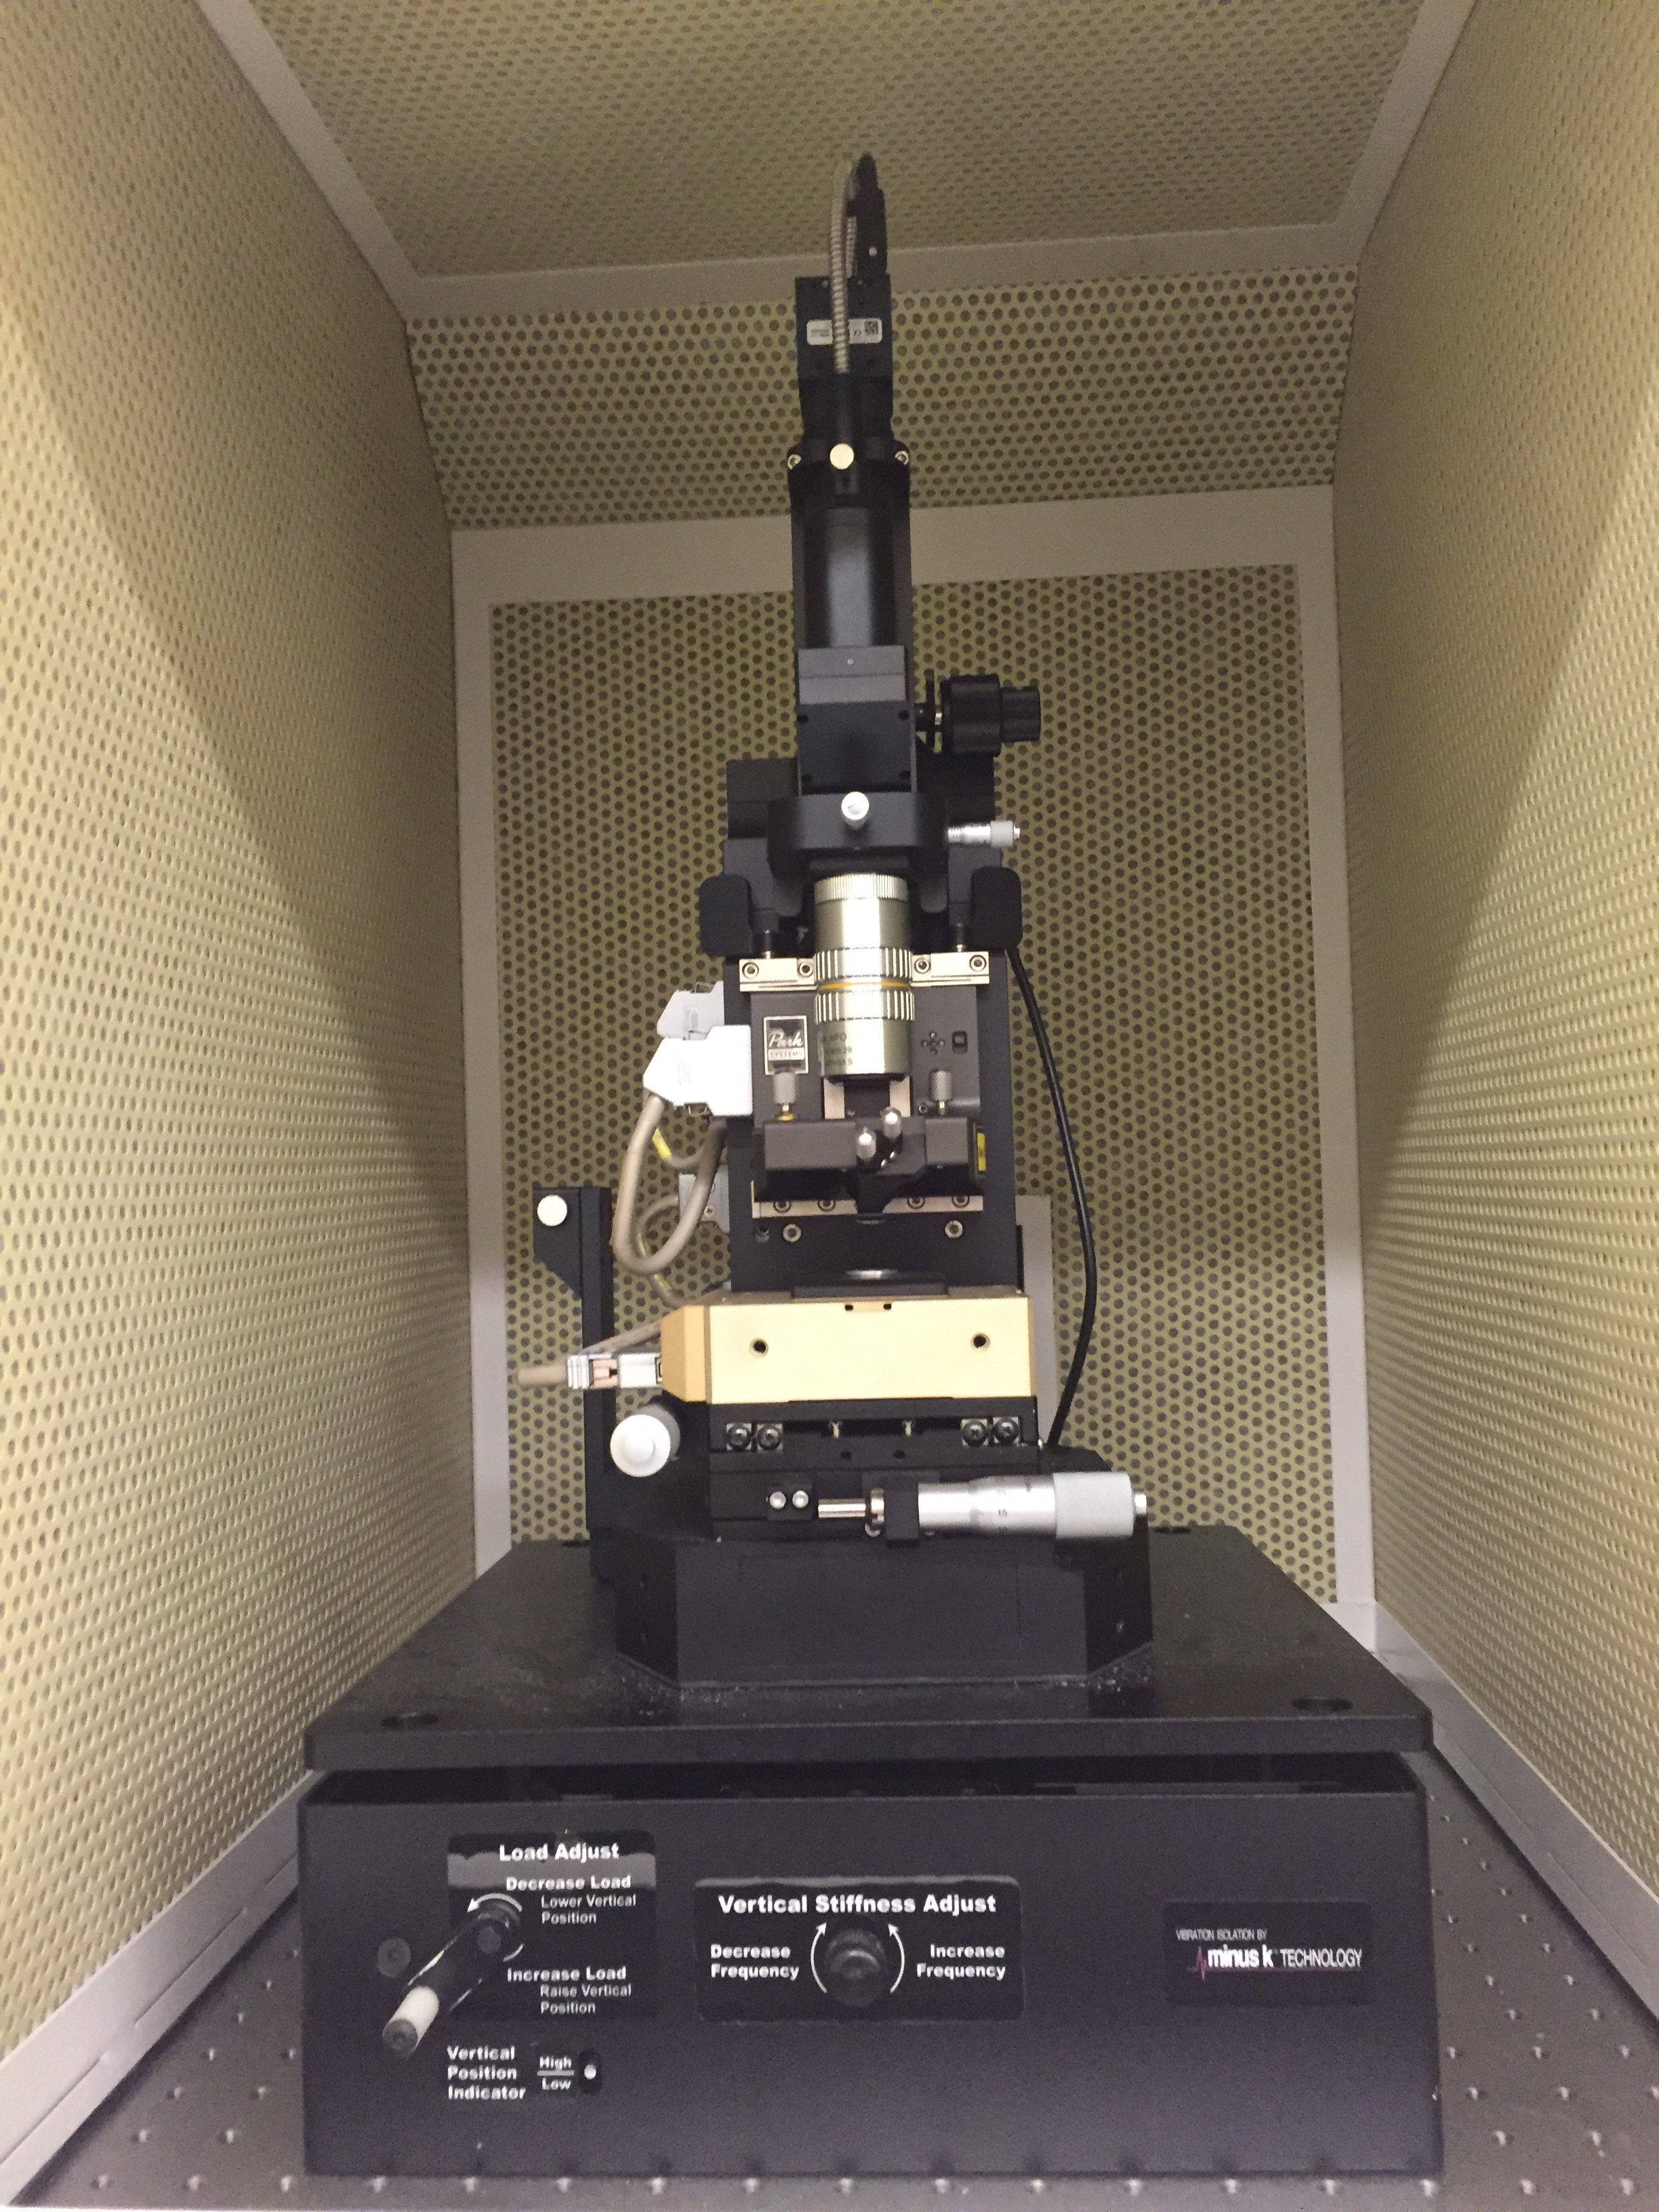
\includegraphics[height=4cm,width=4cm]{figs/experimental/AFM_front_view}
	\caption[AFM front view]{AFM front view}
	\label{fig:afm_front_view}
\end{figure}

\section{Device Fabrication}\label{sec:device_fabrication}
\subsection{Device Design}\label{subsec:device_design}
\subsection{Electron Beam Lithography}\label{subsec:lithography}
\subsection{Metal Deposition}\label{subsec:deposition}


\section{Electrical Measurements}\label{sec:measurements}
\subsection{Measurement Devices}\label{subsec:measurement_devices}
\begin{figure}[ht]
	\centering
	\subfigure[idk1]{
		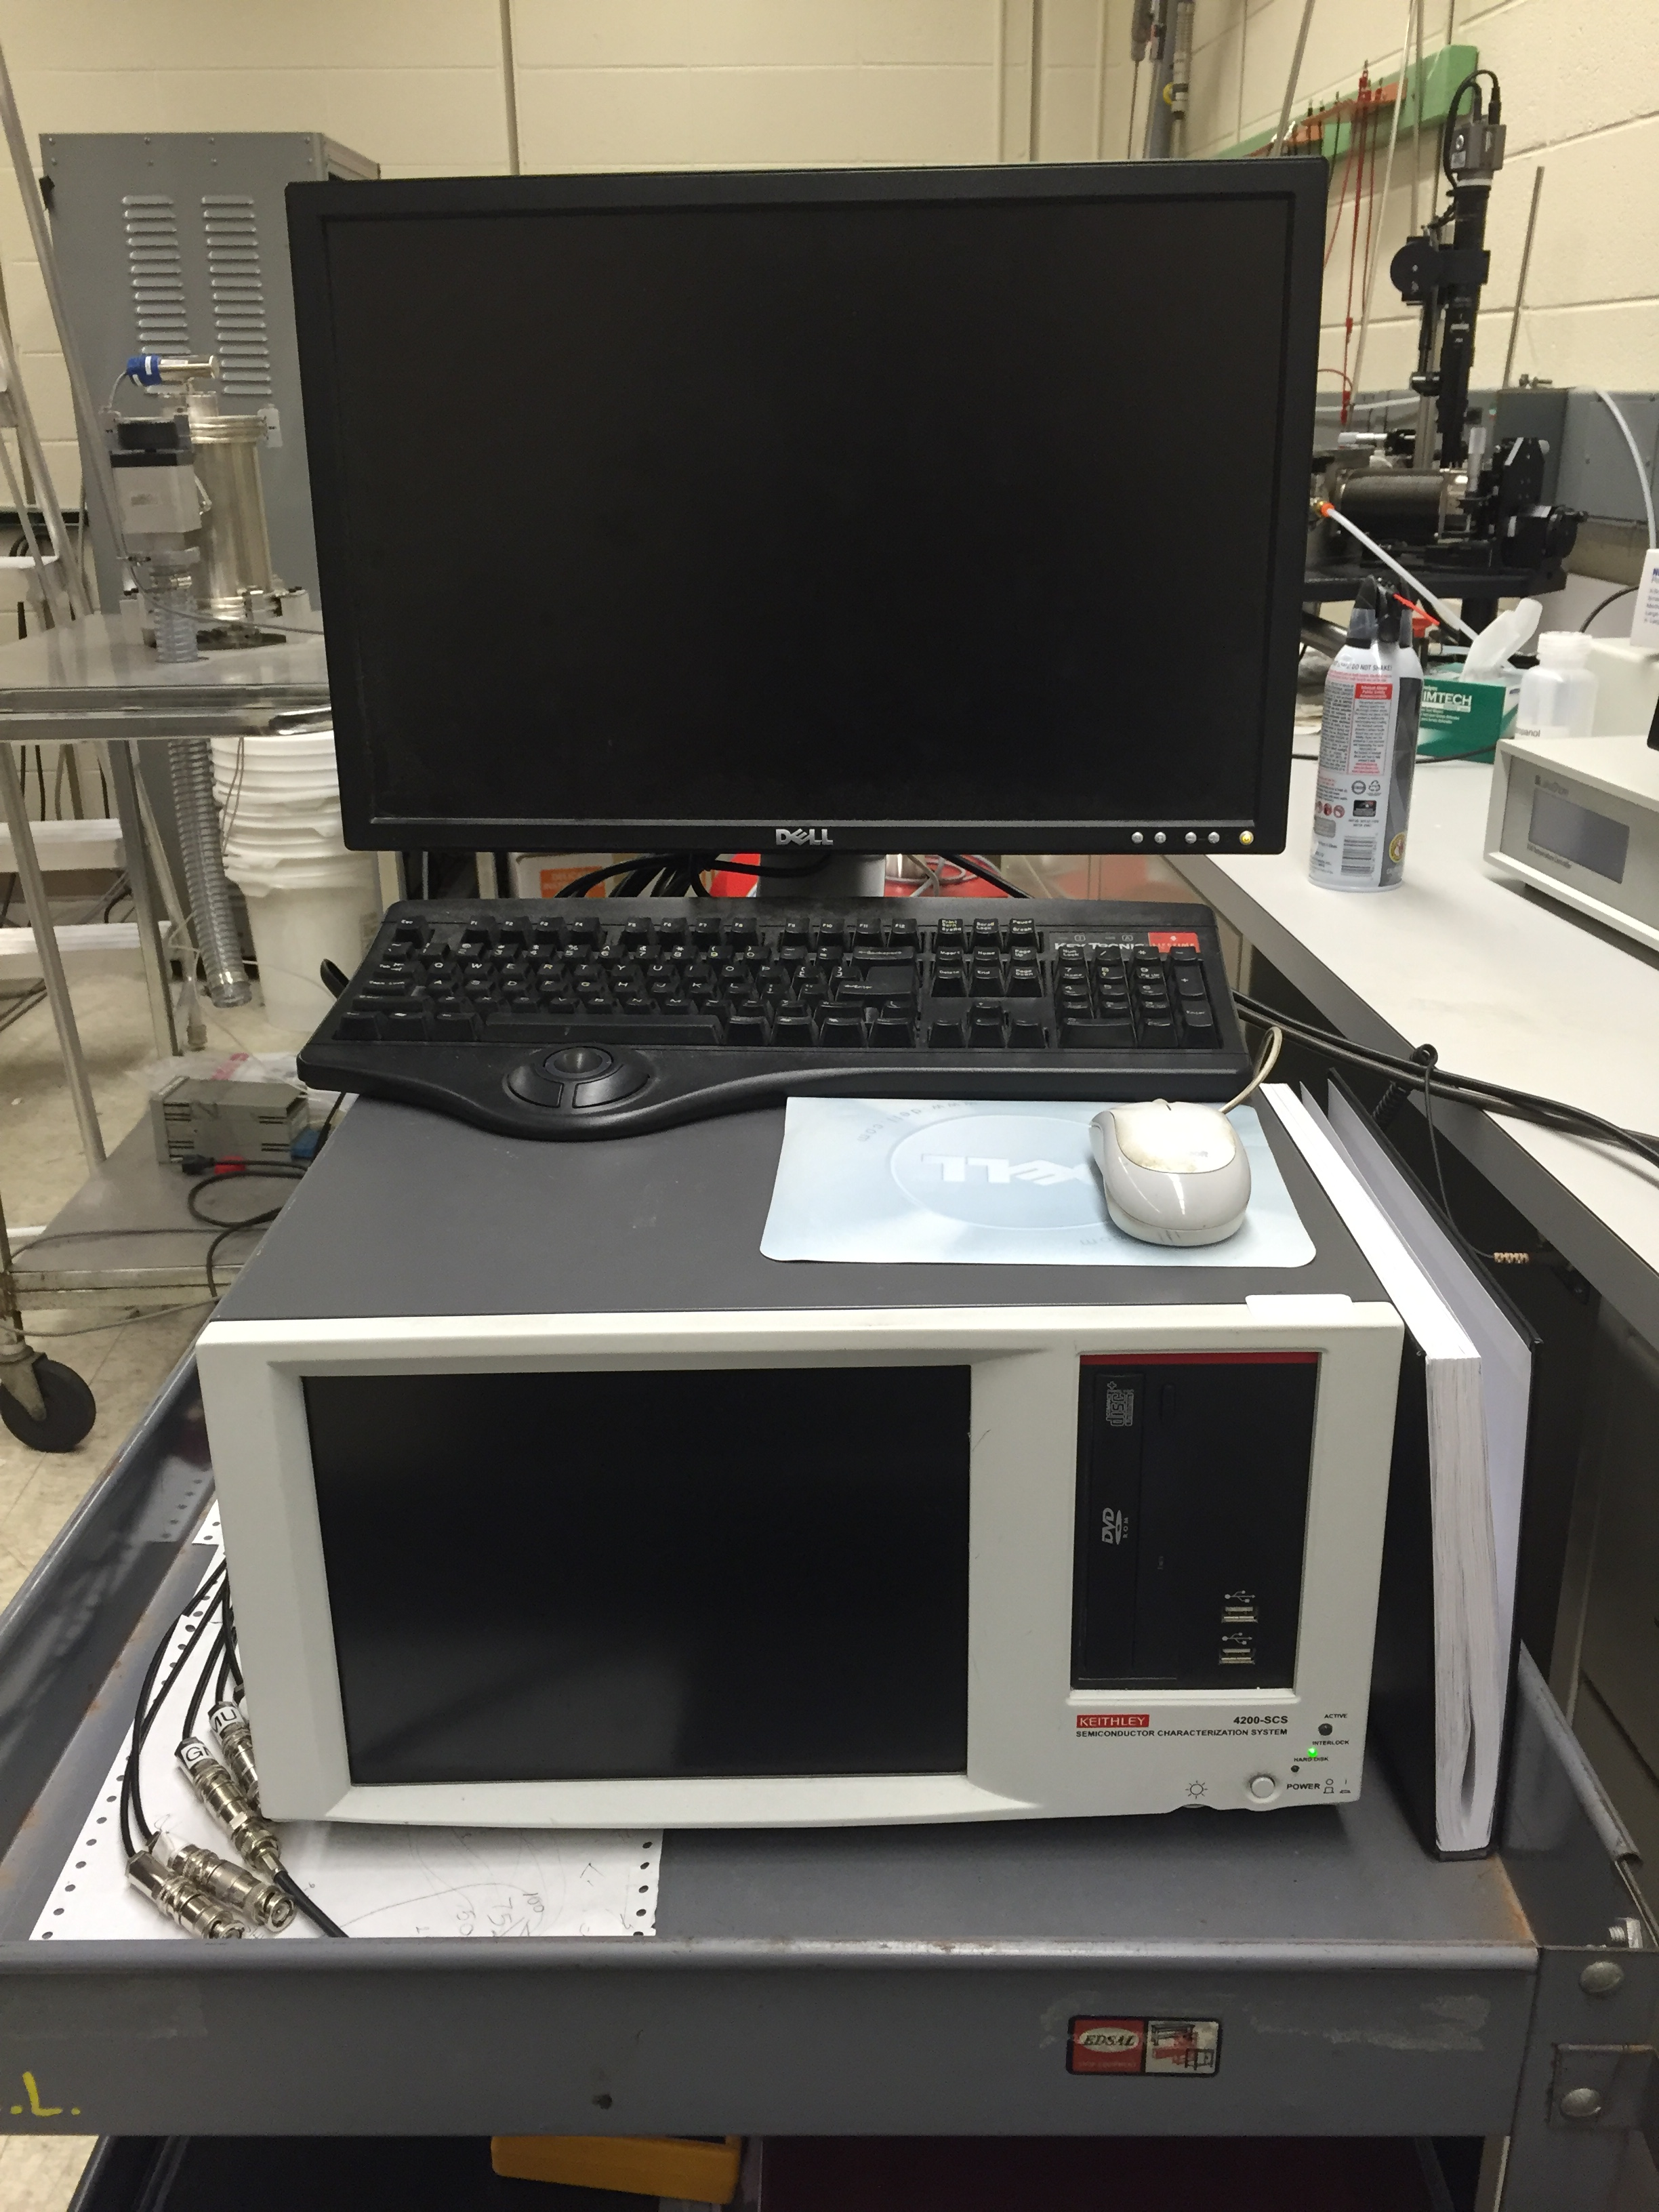
\includegraphics[height=4cm,width=4cm]{figs/experimental/measurement_setup}
		\label{fig:measurement_setup}
	}
	~
	\subfigure[idk2]{
		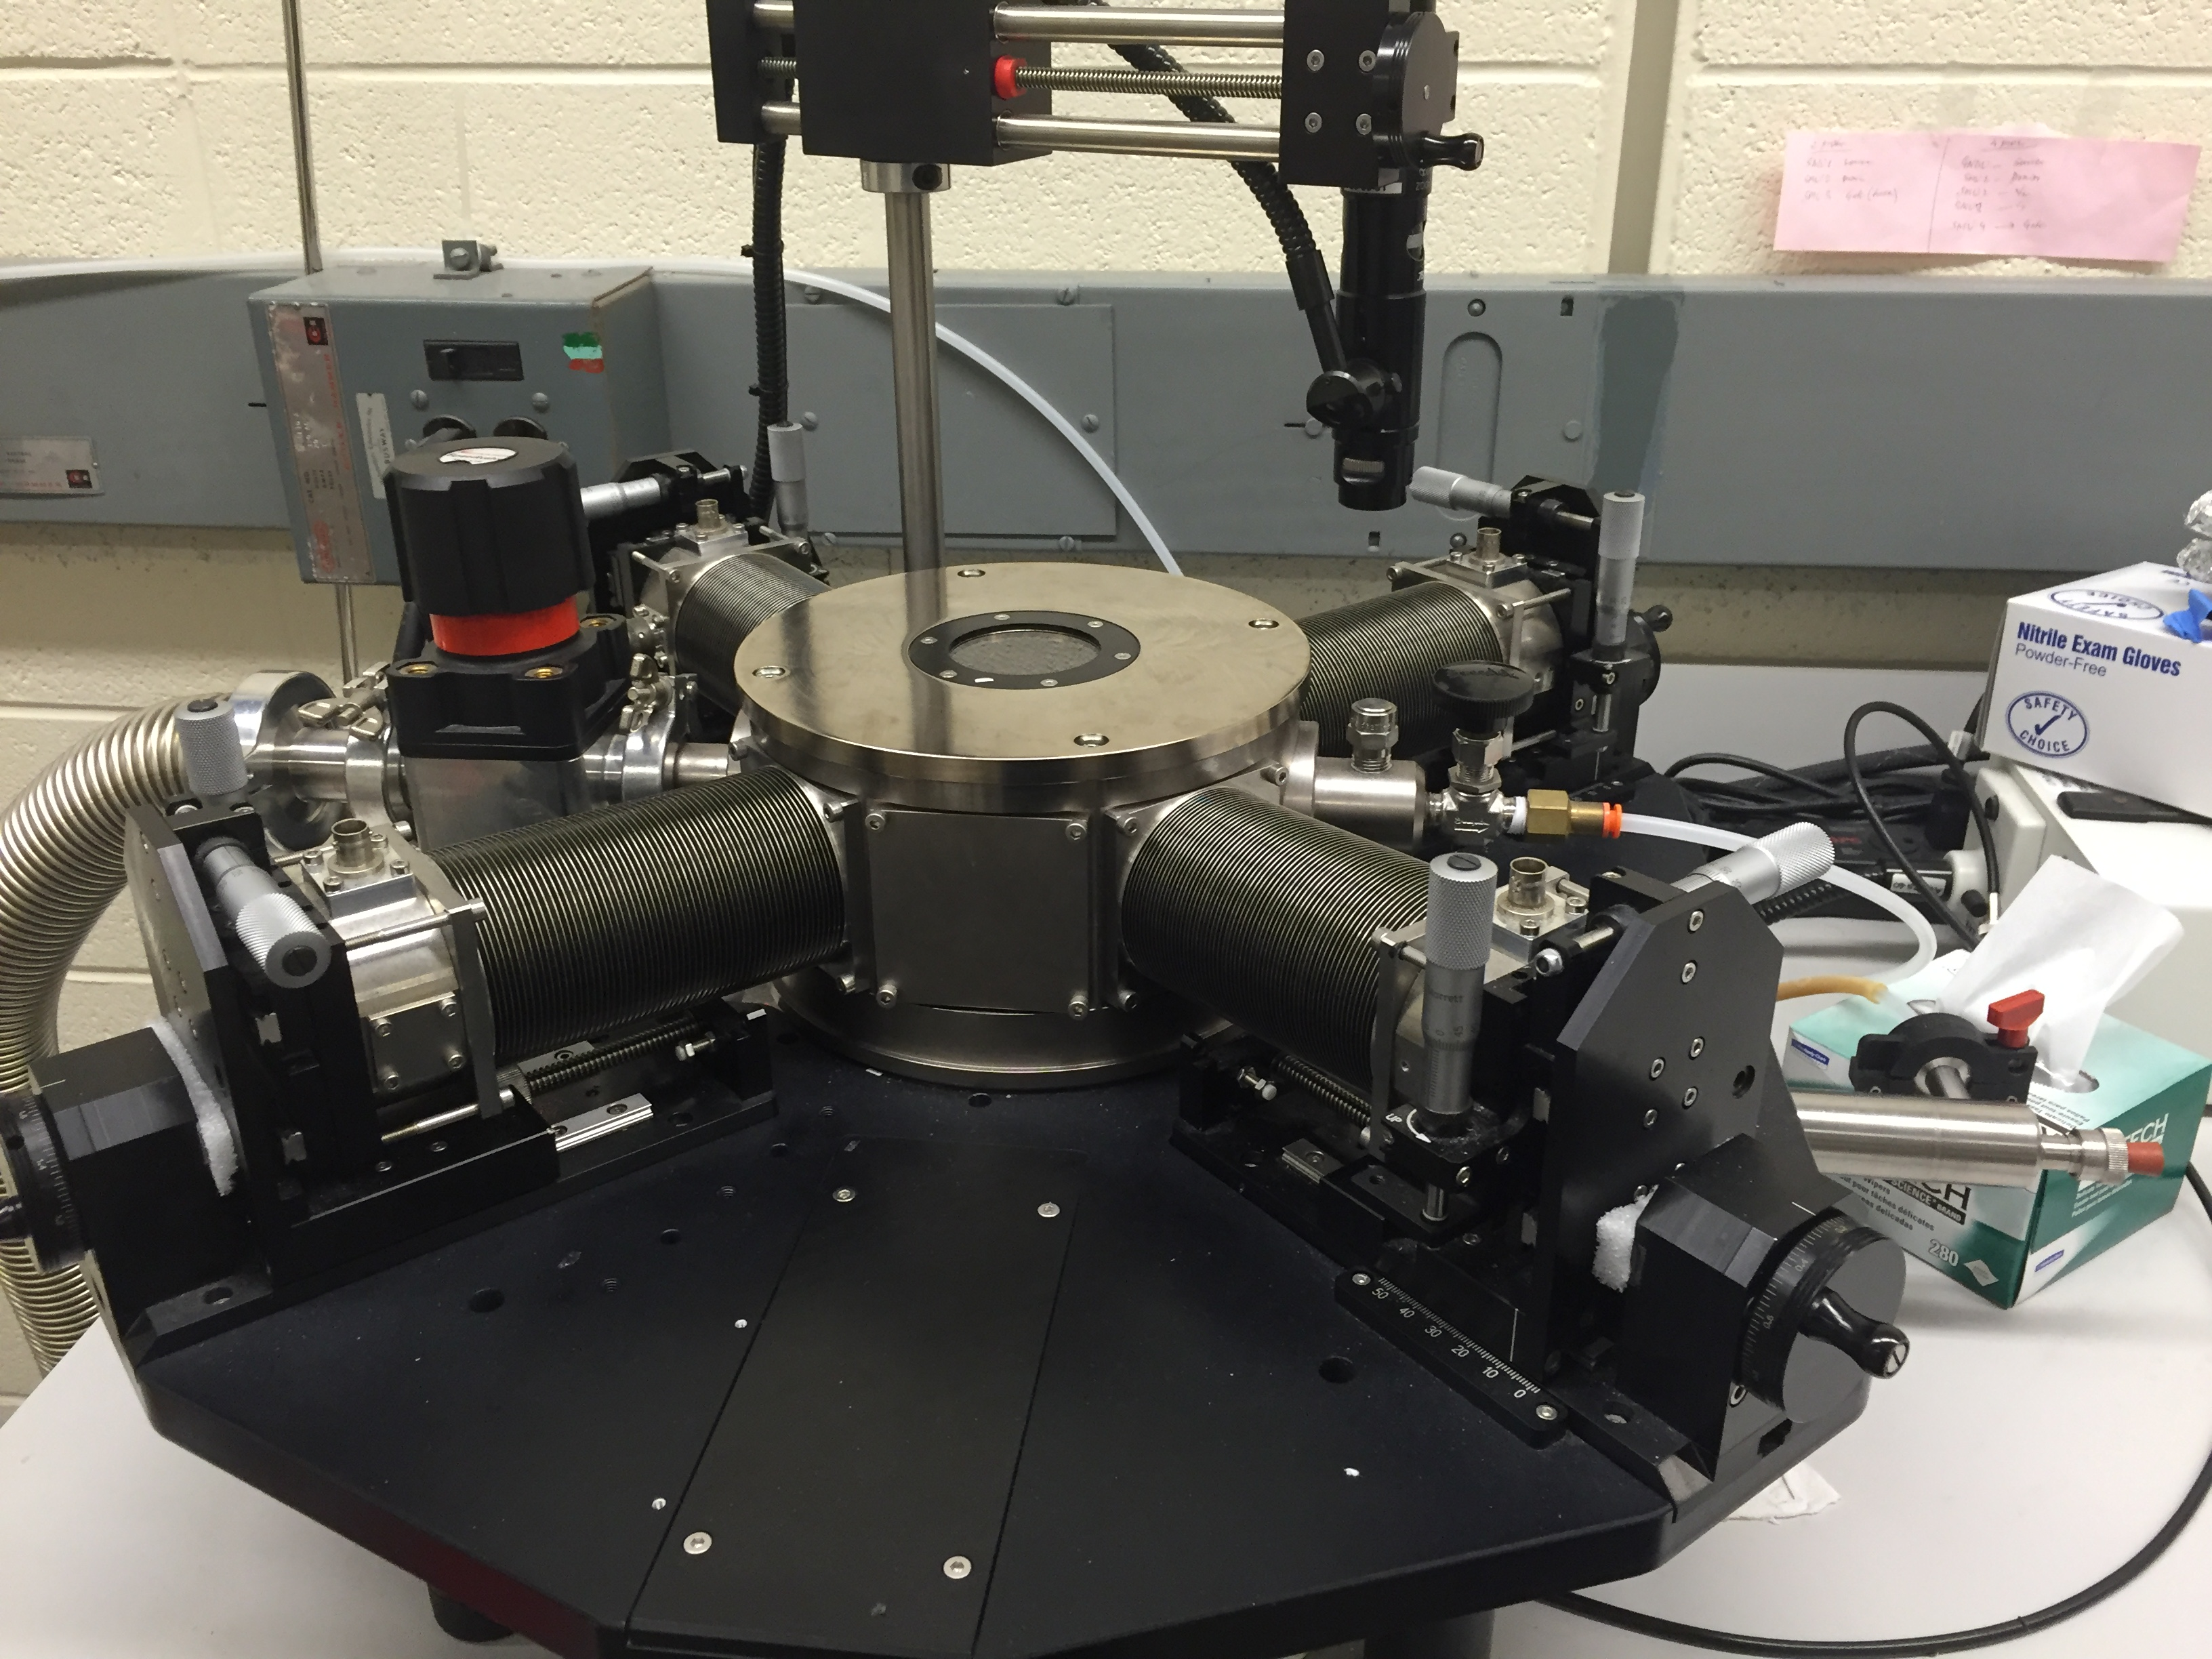
\includegraphics[height=4cm,width=4cm]{figs/experimental/vacuum_measurement}
		\label{fig:vacuum_measurement}
	}
	\caption[Measurement setup]{Main Caption}
	\label{fig:measurement}
\end{figure}
	

